\chapter{Introduction}
\label{chap:Chapter1}

This chapter provides context for automating alert triage and its significance in enhancing security operations in a SOC, particularly for managing high volumes of security alerts. It begins with defining the problem and detailing the challenges associated with manual alert analysis and the critical requirements for automation. First, the objectives of this thesis are presented; second, this project's expected outcomes, including efficiency and accuracy improvements, are outlined, along with the selected approach for integrating an existing ML model to automate alert classification. Finally, an overview of the report's structure is provided.

\section{Context}

In today's world, cybersecurity has become essential for organizations of all sizes. \parencite{Vielberth2020} The rapid advancement of technology, particularly artificial intelligence, has fostered innovation and growth and equipped cybercriminals with increasingly sophisticated tools and techniques. Cyber threats have surged over recent years, and this trend is expected to continue, with global cybersecurity spending projected to rise from \$6 trillion to \$30 trillion by 2030. \parencite{SOVILJ2020113577}

As these threats become more complex and frequent, \gls{SOC} have emerged as the primary line of defense. \gls{SOC}s are crucial in monitoring, detecting, and responding to cyber threats, ensuring the protection of organizations' core digital assets—data, applications, and infrastructure. By combining human expertise with advanced technology, \gls{SOC}s proactively defend systems, respond to incidents, and work to minimize the impact of potential breaches, safeguarding essential operations. \parencite{Jalalvand2024}

However, managing the overwhelming number of alerts generated daily within \gls{SOC}s presents a significant challenge. Analysts must review and respond to thousands of tickets, a process that can quickly lead to burnout, as stated by \textcite{Tines2023}, especially when the majority of alerts are false positives. A study found that many organizations receive over 10,000 alerts daily, with more than 50\% being false positives. \parencite{CriticalStart2019}

One of the stages in the \gls{SOC} workflow with a higher alert volume is the initial triage process. At this stage, Tier 1 analysts are responsible for gathering raw data, assessing alarms, and determining the urgency and nature of each alert. For every ticket, they must evaluate whether the alert is valid or a false positive, assign priority based on the alert’s severity, and identify any potential high-risk incidents. \parencite{Vielberth2020} This process demands significant time and effort, placing a heavy mental load on analysts as they deal with large volumes of information.

Integrating automation in the triage process, particularly for determining alert criticality and classification, could substantially reduce analyst fatigue. \gls{ML} techniques are up-and-coming for processing large data volumes. They facilitate the classification and prioritization of alerts, enabling analysts to focus on high-priority threats. \parencite{Jalalvand2024}

This work explores how \gls{SOC}s can use automation and \gls{ML} to streamline alert triage, improve \gls{SOC} efficiency, and more effectively protect organizations from an ever-evolving cyber threat landscape.

%-------------------------------------------------------------------------------
\section{Problem}

The main objective of this work is to develop an independent program that automates the triage of security alerts within a Security Operations Center (SOC) environment. This automation aims to enhance the overall efficiency and accuracy of the triage process, reduce the number of false positives, and alleviate the workload during the initial stages of the SOC workflow.

Improving the speed of analyzing initial alerts is crucial in a Security Operations Center (SOC) workflow. Faster analysis enables SOC analysts to respond to incidents quickly, which helps minimize the time that threats remain undetected. Without automation, this initial alert analysis depends heavily on manual inspection. Analysts face the challenge of sifting through a large volume of alerts to identify potential threats, which is time-consuming and susceptible to human error. 

This reactive, manual method increases response times and raises the risk of missing critical threats. Analysts must manually classify alerts, assess their severity, and determine appropriate response actions while managing a continuous influx of new alerts. This approach can strain resources and often leads to alert fatigue, making it difficult for analysts to prioritize and respond effectively.

Key metrics such as Mean Time to Detect (MTTD) and Mean Time to Respond (MTTR) can significantly improve by reducing the time required for initial analysis. These metrics are essential for maintaining strong cybersecurity defenses. Automation in alert triage allows for faster and more accurate threat identification, enabling analysts to focus on high-priority threats. This not only increases overall productivity but also reduces fatigue among analysts, while boosting the effectiveness of cybersecurity.

This efficiency results in a more manageable workload, decreased burnout, and greater job satisfaction for employees. For the organization, streamlined response times enhance the security posture, lower the risk of breaches, and ultimately protect critical assets more effectively.

%-------------------------------------------------------------------------------
\section{Objectives}

The objectives for this project are as follows:

\begin{enumerate}
    \item Literature search and review
    \label{objective1}
    \begin{itemize}
        \item A research into the latest advancements in security analysis and a thorough analysis of the tools, methodologies, and approaches researchers use in SOC automation and machine learning applications.
    \end{itemize}
    
    \item Study of existing Machine Learning (ML) models
    \label{objective2}
    \begin{itemize}
        \item An analysis of different models for alert triage in SOC environments and related fields, aiming to identify and improve the adopted approach.
    \end{itemize}
    
    \item Collection of security alert datasets
    \label{objective3}
    \begin{itemize}
        \item A compilation of accessible datasets on security alerts organized to supply training data for the selected ML model.
    \end{itemize}

    \item Integration with SIEM and other data sources
    \label{objective4}
    \begin{itemize}
        \item Connect the SIEM and relevant data sources for real-time data ingestion and analysis.
    \end{itemize}
    
    \item Developing a custom dashboard for analysts to submit feedback on the machine learning model.
    \label{objective5}
    \begin{itemize}
        \item While the ML model will be trained with existing datasets before deployment, it is still beneficial to provide a method for analysts to continue training the model over time.
    \end{itemize}
    
    \item Testing and evaluation of the selected ML model
    \label{objective6}
    \begin{itemize}
        \item The selected ML model will be tested with live data, followed by an analysis to assess its effectiveness in categorizing alerts and minimizing false positives.
    \end{itemize}
\end{enumerate}

\section{Research Contextualization}

This research will be conducted at ArtResilia, a cybersecurity firm dedicated to improving organizational cyber resilience through proactive threat anticipation, strong security measures, and efficient recovery.
As they emphasize: 

\begin{quote}
    "Everyone will be attacked someday, what matters is how fast they recover!"  
\end{quote}

This reflects their focus on minimizing the impact of cyber threats and enabling organizations to maintain operational continuity \parencite{artresilia2024}.

ArtResilia offers a broad range of cybersecurity services divided into three main areas:
\begin{itemize}
    \item \textbf{Defensive Security:} Design, implementation, and management of security solutions. Their state-of-the-art Security Operations Center (SOC), known as Helix, provides end-to-end security operations, including threat anticipation, detection, protection, and incident recovery.
    \item \textbf{Offensive Security:} Comprehensive testing and validation of organizational assets by simulating real-world threat actor techniques, including penetration testing, threat intelligence, and deception-based strategies.
    \item \textbf{Advisory Services:} Consulting services focused on governance, risk management, compliance (GRC), and security architecture to ensure organizations meet regulatory and operational security requirements.
\end{itemize}

ArtResilia was approached for a research project exploring strategies to enhance cybersecurity resilience through automation and machine learning. The project aligns with ArtResilia's mission to strengthen incident detection and response capabilities against emerging cyber threats.

After reviewing the proposal, ArtResilia accepted the project and committed to providing support and resources for its implementation. This collaboration underscores ArtResilia's dedication to fostering cybersecurity innovation and ensuring real-world applications in professional security operations.

\section{Research Questions}

For this research, three key research questions (RQs) were devised to address the central issue of improving the efficiency and accuracy of security alert triage within Security Operations Centers (SOCs). 
Each question offers a targeted perspective for examining specific facets of the problem, contributing to the overarching objective of minimizing both false positives and false negatives in security alerts. 
Below are the RQs, along with a brief discussion of their significance.

\begin{enumerate}
    \item \textbf{How can ML techniques be applied to the triage of security alerts to reduce false positives and negatives?} \\
    This question explores how machine learning (ML) can tackle the challenge of excessive alerts in SOCs, characterized by high false positive and negative rates. The goal is to identify effective ML techniques and assess their impact on improving alert accuracy.
    
    \item \textbf{What are the main challenges in implementing an AI bot integrated with SIEM systems, and how can they be mitigated?} \\
    Implementing AI in security systems presents a range of challenges, from broader issues like data integration, system compatibility, and performance maintenance under varying conditions, to narrower challenges such as trusting the AI to serve as an advisor to the manual work of the SOC analyst. It's also crucial to ensure that the percentage of incorrect classifications does not jeopardize trust in the solution. This research question aims to identify these challenges and propose strategies for successful AI integration.
        
    \item \textbf{What ML frameworks and methodologies exist, and which are most suitable for developing and training AI models for ticket triage in SOC environments?} \\
    Understanding ML frameworks and methodologies is essential for choosing the right tools for AI model development in SOC ticket triage. This question examines the suitability of different frameworks based on their capabilities and alignment with SOC needs.
\end{enumerate}

To answer these research questions systematically and comprehensively, a structured approach was adopted. 
This approach involved defining keywords, utilizing relevant digital libraries, and employing robust frameworks for the literature review.

The following keywords and their combinations were used to identify relevant papers:
\begin{itemize}
    \item \textbf{Keywords:} Machine learning, AI, security alerts, SOCs, SIEM systems
    \item \textbf{Keywords:} False positives, false negatives, alert triage, alert fatigue
    \item \textbf{Keywords:} AI integration, ticket prioritization, frameworks, methodologies
\end{itemize}

The primary digital libraries used were:
\begin{itemize}
    \item \textbf{ACM Digital Library}: For accessing peer-reviewed articles on machine learning and security applications.
    \item \textbf{ResearchGate}: For exploring academic discussions, preprints, and supplementary materials.
\end{itemize}

Search strings using these keywords were used to search the digital libraries effectively.
\begin{itemize}
    \item \textbf{Search String 1:} ("Machine learning" AND "security alerts") AND ("false positives" OR "false negatives")
    \item \textbf{Search String 2:} ("AI integration" AND "SIEM systems") OR ("ticket prioritization")
    \item \textbf{Search String 3:} ("Frameworks" AND "SOC environments") AND ("alert triage")
\end{itemize}

In addition to the search strings, a new constraint was implemented to limit the findings to the most recent five years, ensuring the collection of up-to-date research and information.

To structure my literature review, two complementary frameworks were used: \textbf{PICOCS} and \textbf{snowballing}.

\begin{itemize}
    \item \textbf{PICOCS Framework}: This framework helped define the Population, Intervention, Comparison, Outcome, Context, and Study type for each RQ as can be seen on Figure~\ref{tab:picocs_rqs}. Using PICOCS ensured a focused and systematic approach to identifying papers aligned with this research objectives.

\captionsetup[table]{font=small} % Set the caption font size
\scriptsize % Reduce the font size for the table content
\begin{longtable}{p{1cm}p{1.5cm}p{3cm}p{3cm}p{3cm}}
    \caption{PICOCS Framework for Research Questions}
    \label{tab:picocs_rqs} \\
    \toprule
    \textbf{Element} & \textbf{Definition} & \textbf{RQ1} & \textbf{RQ2} & \textbf{RQ3} \\
    \midrule
    \endfirsthead
    \toprule
    \textbf{Element} & \textbf{Definition} & \textbf{RQ1} & \textbf{RQ2} & \textbf{RQ3} \\
    \midrule
    \endhead
    \bottomrule
    \endfoot
    \bottomrule
    \endlastfoot
    P & Population & SOC analysts dealing with alerts & SOC analysts and SIEM administrators & SOC analysts developing AI models \\
    I & Intervention & Machine learning techniques & AI bots integrated with SIEM systems & ML frameworks and methodologies \\
    C & Comparison & Manual triage methods & Existing rule-based systems & Alternative ML frameworks \\
    O & Outcome & Reduction in false positives/negatives & Mitigation of integration challenges & Identification of suitable frameworks \\
    C & Context & SOC environments & SOC environments using SIEM systems & SOC environments implementing AI models \\
    S & Study Type & Empirical studies, experiments & Case studies, technical reports & Framework evaluations, experiments \\
\end{longtable}

\normalsize

    \item \textbf{Snowballing Method}: Starting with an initial set of highly relevant papers, I used snowballing to identify additional studies by exploring their references (backward snowballing) and citations (forward snowballing). This iterative process expanded the breadth of my review.
\end{itemize}
    
\paragraph{Combining PICOCS and Snowballing} The combination of PICOCS and snowballing provided a balance between structure and adaptability. 
PICOCS ensured a methodical and targeted search, while snowballing allowed for iterative exploration beyond initial search results, capturing emerging trends and overlooked studies.

By following this approach, it was possible to systematically answered the RQs and developed insights that directly contribute to improving the triage of security alerts in SOC environments.

% WBS not needed for DIMEI
% \section{Work Breakdown Structure}

% Figure~\ref{fig:wbs-image} represents a detailed WBS for this research.

% \clearpage

% \begin{figure}[htp]
%     \centering
%     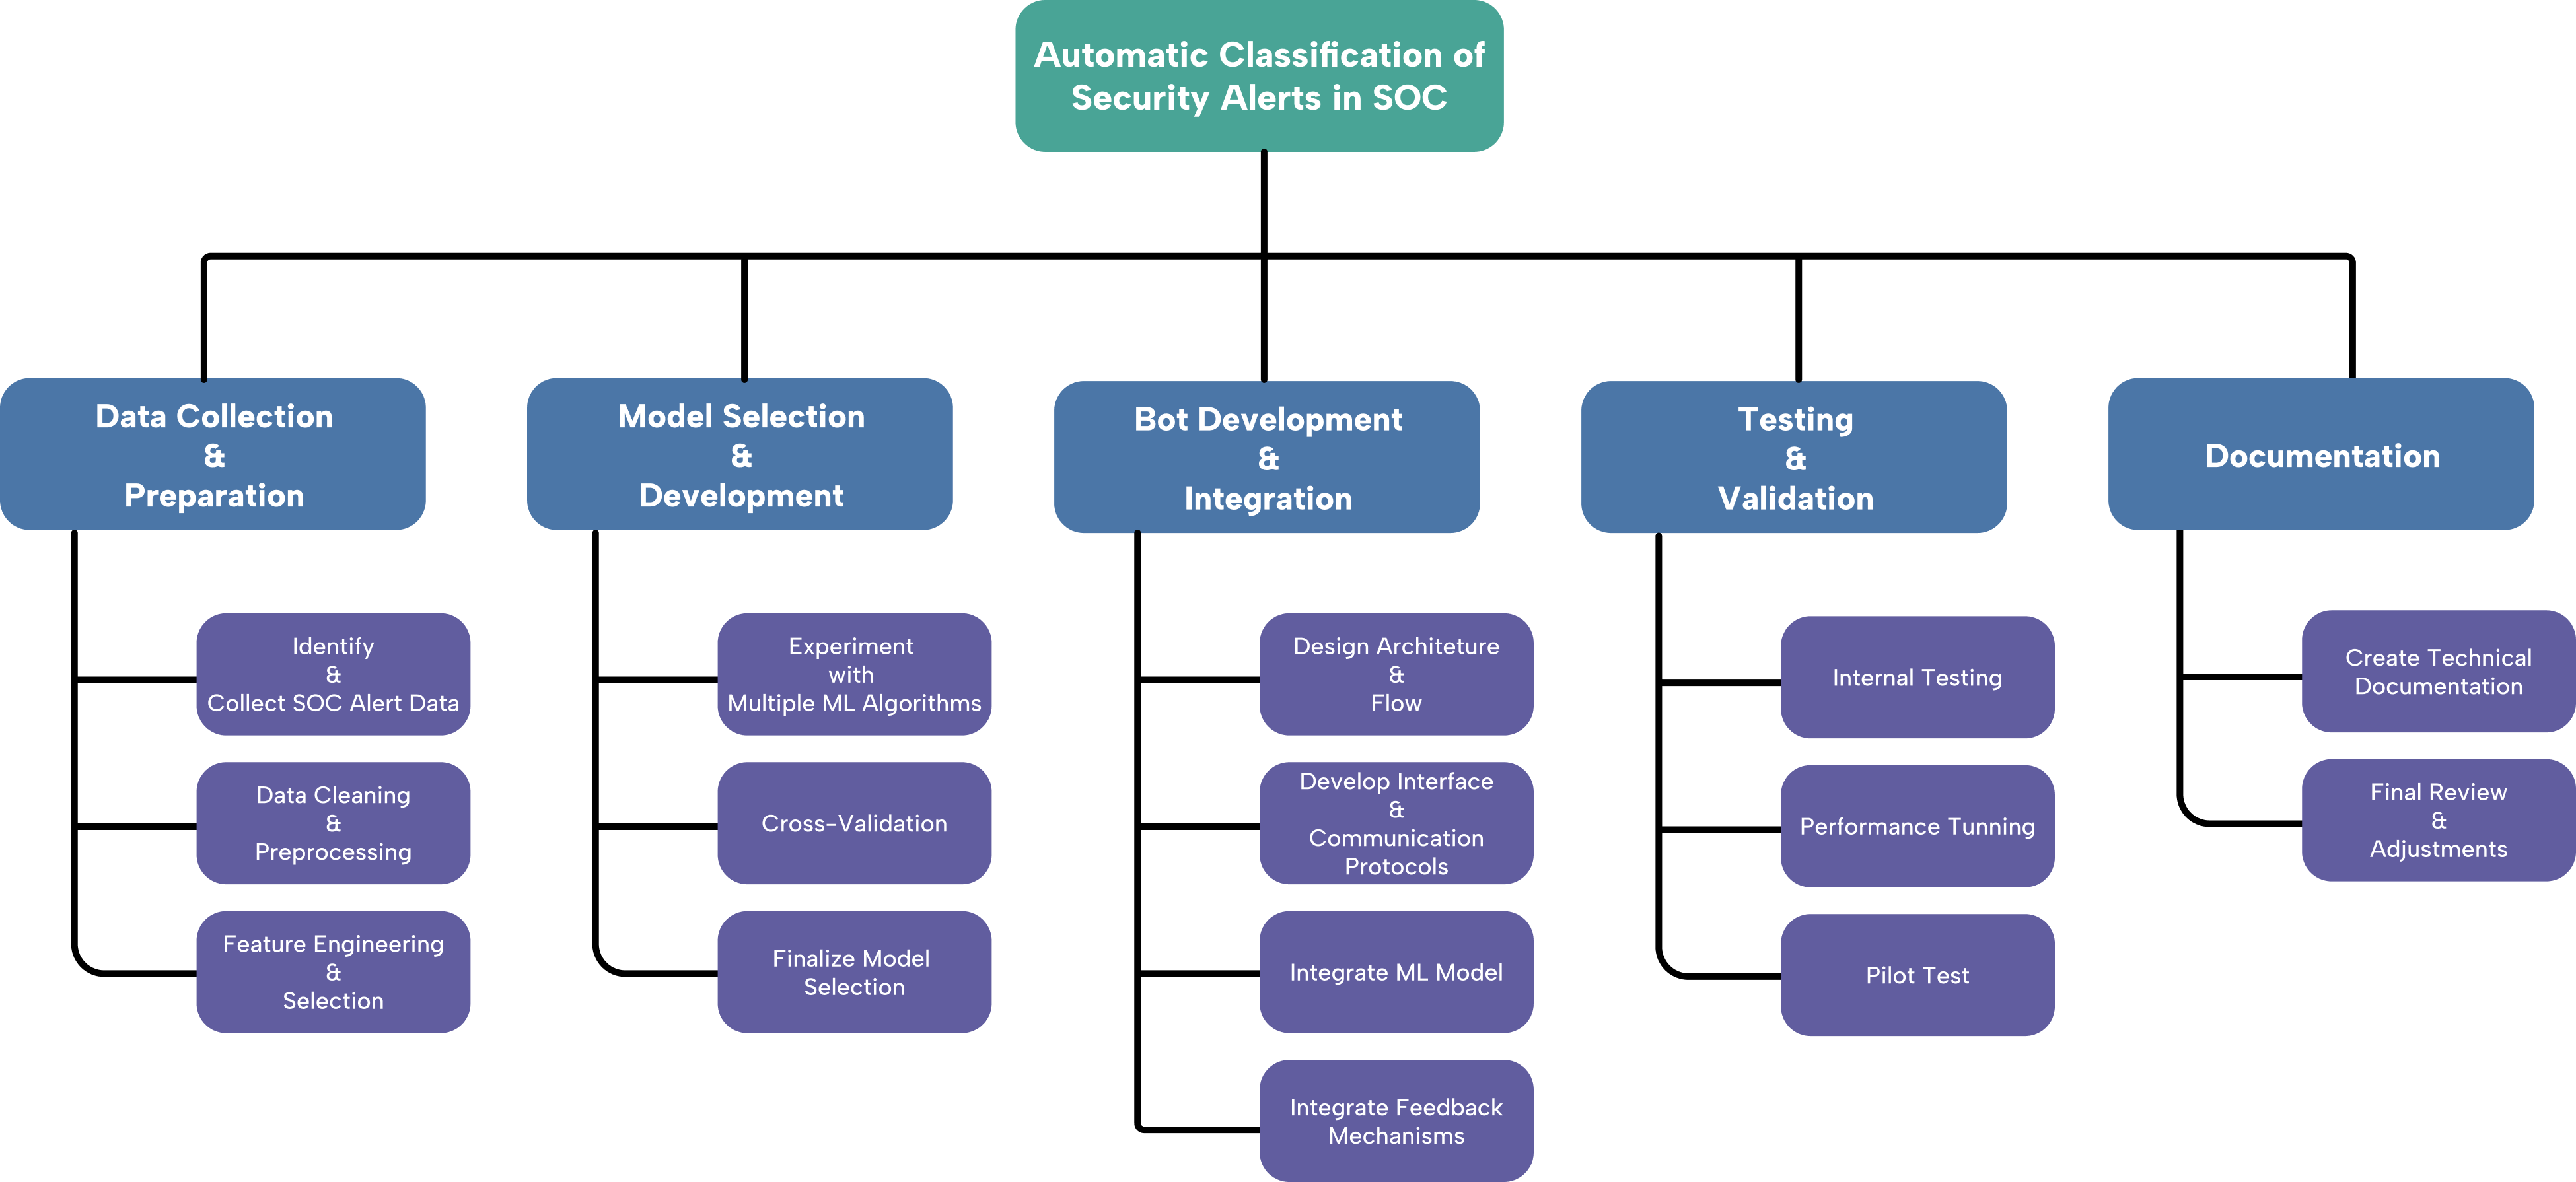
\includegraphics[scale=0.18, angle=270]{ch1/assets/WBS.png}
%     \caption{Work Breakdown Structure}
%     \label{fig:wbs-image} 
% \end{figure}

% \clearpage

%-------------------------------------------------------------------------------
\section{Dissertation Structure}

This dissertation is organized into five chapters, each addressing a key component of the research process and contributing to the overall objective of developing an automated security alert triage system for \gls{SOC}.

\begin{itemize}
    \item \textbf{Chapter 1 - Introduction}: Presents the context, motivation, and objectives of the research. It introduces the problem statement, research questions, and the organizational environment where the study was conducted.
    \item \textbf{Chapter 2 - State of the Art}: Provides a comprehensive literature review covering the foundations of Security Operations Centers, Security Information and Event Management (SIEM) systems, Machine Learning techniques, and existing approaches to automated alert classification. It also includes a comparative analysis of relevant technologies.
    \item \textbf{Chapter 3 - Method and Implementation}: Describes the methodological approach adopted, including the technological choices, the proposed solutions, and the architectural design. It details the implementation steps, dataset preparation, model development, and system integration.
    \item \textbf{Chapter 4 - Model Evaluation and Results Analysis}: Presents the experimental evaluation of the developed system, discussing both local and live testing environments, performance metrics, and a detailed analysis of the obtained results.
    \item \textbf{Chapter 5 - Conclusion and Future Work}: Summarizes the main findings of the research, reflects on its contributions and limitations, and proposes potential directions for future work to enhance and extend the developed solution.
\end{itemize}


\section{Ethical Considerations}

During the writing of this dissertation, AI-powered features of Grammarly were used to support the revision and improvement of the text. 
This included grammar correction, clarity suggestions, and occasional rephrasing to enhance readability and coherence.

No content generated by AI contributed to the research results, technical implementation, or core arguments of this work. 
The use of AI was strictly limited to language polishing and did not influence the academic or scientific content in any way.

%-------------------------------------------------------------------------------
%---------
%